\documentclass[Rapport/Rapport_main.tex]{subfiles}
\begin{document}
\section{Indledning}\label{sec:Indledning}
\subsection{Motivation og kontekst}
Beer Pong er et spil, der ofte udgør samlingspunktet ved festlige lejligheder og i sociale sammenhænge. Alkoholindtag og konkurrencer hænger uløseligt sammen, og Beer Pong formår at kombinere disse på en måde, som har gjort det til et af tidens mest populære og udbredte drukspil.\textcolor{orange}{ref} \\\\Det spilles typisk af to konkurrerende hold, som hver består af 2 spillere. Holdene står i hver deres ende af et aflangt bord og kaster på skift en bordtennisbold hen over bordet, med det formål at ramme ned i modstanderens kopper. Kopperne indeholder øl og er placeret i trekantede formationer af 6 kopper i hver ende af bordet. Når bolden lander i en kop, indtages indholdet af modstanderen, og koppen fjernes fra bordet. Vinderen er det hold, som først eliminerer alle modstanderens kopper.\textcolor{orange}{ref}
\\\\Beer Pong findes i forskellige varianter, men fællesnævneren for mange af spillene er simple og primitive borde. Det medfører ofte, at der opstår tvivl omkring spillets score, og om en given kop er ramt eller ej. Da det er brugernes eget ansvar at styre spillets gang, hersker der ofte udbredt forvirring. Der er således behov for et produkt, som hjælper med at styre spillets gang og giver visuel respons samt information om spillets status.
\\\\Dette projektarbejde tager udgangspunkt i projektoplægget til 3. semester E/IKT\cite{Universitet2018}. Der arbejdes derfor efter en SCRUM baseret proces, hvor semesterets kurser integreres. Formålet er at implementere og teste et udviklingsprojekt, som kombinerer både HW og SW. Det udviklede produkt skal basere sig på en indlejret Linux platform og PSoC platform. Der er fokuseret på, at produktet skal interagere med omverdenen gennem anvendelsen af sensorer/aktuatorer, og desuden skal det have et brugerinterface.\\\\

\subsection{Hvad er og kan vores system?}
Systemet som ønskes udviklet er en forbedret og interaktiv udgave af et Beer Pong bord. For at sikre en forbedret brugeroplevelse er der lagt stor vægt på, at bordet skal give spillerne en form for visuel feedback. Dette skal blandt andet komme fra belysning under kopperne. Lyset kan antage mange forskellige farver og styres individuelt for den enkelte kop. Det varierer afhængigt af, om der er placeret en kop eller ej, og det giver udslag, når en bordtennisbold rammer ned i koppen. Der anvendes sensorer under hver kop, for netop at detektere om der er en kop placeret, og om den er ramt af en bordtennisbold.\\\\Via et møntindkast kan bordet modtage danske 5-kroner. Når den korrekte mønt detekteres, skal en dispenser i bordet forsyne spillerne med en bordtennisbold. To lysdioder informerer om antallet af bordtennisbolde i dispenseren. Når en sensor detekterer, at der er færre end 2 bolde tilbage, lyses der rødt frem for grønt.\\\\For at sikre en endnu større grad af brugerinteraktion, får spillerne mulighed for at tilgå et WiFi-netværk med smartphone, eller et andet mobilt device. Her indtastes brugernavne, holdnavne og holdfarve. Holdfarven kommer til udtryk i lysene i Playerside, mens navnene kommer til at fremgå af et display. Dette display skal desuden vise antallet af tilbageværende kopper, og det opdateres løbende under spillet. Foruden underholdningsværdien sikrer det, at alle kan følge med i spillets gang, og at overblikket bevares.

\subsection{Hvor kan systemet realiseres?}
Bordet indeholder alle de platforme og elementer, som skal til for at spille. Det ville derfor være nemt at installere, da det kun skal kobles til en stikkontakt. Desuden skal der indsættes en mønt i bordet, før man kan få en bold og starte spillet, så det vil være oplagt at anbringe bordet et offentligt sted som en bar eller en klub, hvor man ønsker den komplette Beer Pong oplevelse.

\subsection{Projektformulering}
Målet for dette projekt er at udarbejde en funktionel prototype af et Beer Pong bord. Bordet skal være baseret på en indlejret Linux platform og en PSoC platform. Sensorer skal anvendes til at registrere indsatte mønter, anbringelse og fjernelse af kopper samt hændelsen at en bordtennisbold rammer ned i en kop. En aktuator skal anvendes til at dispensere bordtennisbolde. Bordet skal have mindst seks kopholdere med lys under hver kop. Det skal være muligt at tilgå en hjemmeside og indtaste holdnavne, brugernavne og holdfarver. Holdfarver skal fremgå af farven på lyset under kopperne, og navnene skal vises på et brugerinterface i form af et display. Display viser desuden holdenes score og opdateres løbende under spillet. Det samlede system kombinerer således sensorer, aktuatorer og brugerinterfaces i et interaktivt og underholdende Beer Pong bord for at sikre den bedst mulige brugeroplevelse.

\subsubsection{Skitse af system}
Figur \ref{fig:system_skitse} viser en grafisk repræsentation af systemet. På figuren er vist et fuldt bord med to Player sides. Hver player side består af seks kopholdere, som hver indeholder lys og sensorer. Ball dispenser indeholder dispenser og møntindkast. Logikken for disse dele af systemet varetages af en PSoC 5LP. Display er vist i midten og styres sammen med webserver af en RPi Zero W. RPi er også forbundet til førnævnte delsystemer, og er essentiel i forhold til afviklingen af spillet og styring af hele systemets logik.

\begin{figure}[H]
    \centering
    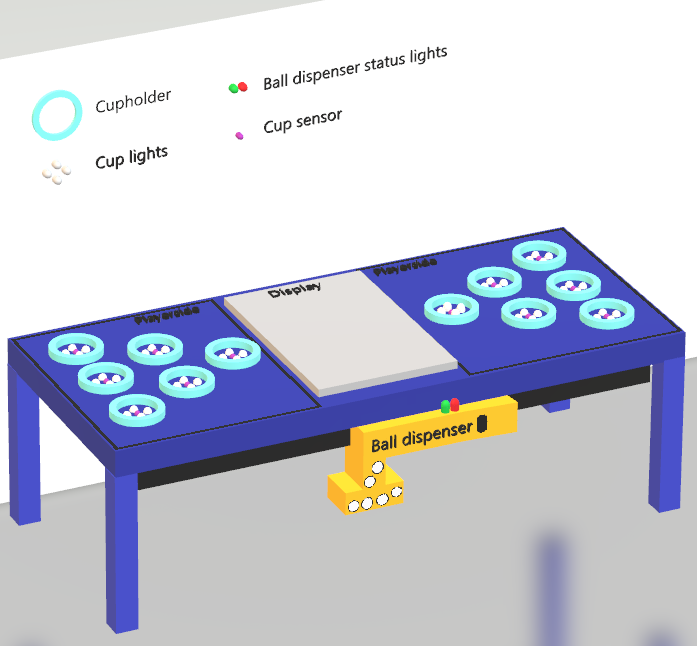
\includegraphics[width=0.9\textwidth]{Rapport/Indledning/graphics/system_skitse.png}
    \caption{Skitse af Beer Pong Table}
    \label{fig:system_skitse}
\end{figure}

\subsection{Ansvarsområder}
I dette afsnit beskrives ansvarsområder samt arbejdsfordeling for udfærdigelse af projektet. Ansvarsområderne er inddelt i primære og sekundære. Primære ansvarsområder indebærer den største arbejdsindsats samt ansvar for, at det bliver færdiggjort rettidigt. Sekundære ansvarsområder indebærer en hjælpende eller mindre indsats uden ansvar for, at det bliver færdiggjort i tide. Fordelingen fremgår af tabellerne nedenfor.

\begin{table}[H]
\centering
\begin{tabular}{|L{0.3\textwidth}|L{0.3\textwidth}|L{0.3\textwidth}|}
\hline
\textbf{Navn} & \textbf{Primær} & \textbf{Sekundær} \\ \hline
Aaron Sanchez & & \\ \hline
Edward Brunton & & \\ \hline
Marcus Gasberg & & \\ \hline
Martin Jespersen & & \\ \hline
Martin Lundberg & & \\ \hline
Mathias Hansen & & \\ \hline
Nikolaj Gylling & & \\ \hline
Tristan Møller & & \\ \hline
\end{tabular}
\caption{Arbejdsfordeling for hardware}
\label{tab:fordeling_HW}
\end{table}

\begin{table}[H]
\centering
\begin{tabular}{|L{0.3\textwidth}|L{0.3\textwidth}|L{0.3\textwidth}|}
\hline
\textbf{Navn} & \textbf{Primær} & \textbf{Sekundær} \\ \hline
Aaron Sanchez & & \\ \hline
Edward Brunton & & \\ \hline
Marcus Gasberg & & \\ \hline
Martin Jespersen & & \\ \hline
Martin Lundberg & & \\ \hline
Mathias Hansen & & \\ \hline
Nikolaj Gylling & & \\ \hline
Tristan Møller & & \\ \hline
\end{tabular}
\caption{Arbejdsfordeling for software}
\label{tab:fordeling_SW}
\end{table}




\end{document}